\section{Data Processing} \label{sec:data_processing}
We assemble our curated \LaViDa \ dataset by retrieving, from a large pool of uncurated data, images that are close to those in several curated datasets. 
We describe below the main components in our data pipeline including the curated/uncurated data sources, the image deduplication step and the retrieval system. 
Our pipeline does not require any metadata or text and directly works with images, as shown in Fig.~\ref{fig:retrieval-system}. 
We refer the reader to appendix \ref{sec:supp-data} for more details on our approach.

\begin{figure}[t]
  \centering
  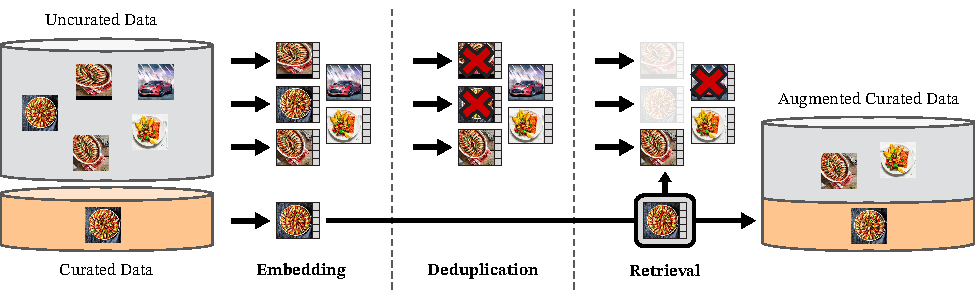
\includegraphics{LaViDa_datapipeline_figure.pdf} 
  \caption{
    \textbf{Overview of our data processing pipeline.} 
    Images from curated and uncurated data sources are first mapped to embeddings. 
    Uncurated images are then deduplicated before being matched to curated images. 
    The resulting combination augments the initial dataset through a self-supervised retrieval system.
  }
  \label{fig:retrieval-system}
\end{figure}

\myparagraph{Data sources.}
Our selection of curated datasets is detailed in the appendix (Table \ref{tab:lavida-details}) and contains ImageNet-22k, the train split of ImageNet-1k, Google Landmarks and several fine-grained datasets.
For the uncurated data source, we collect a raw unfiltered dataset of images from a publicly available repository of crawled web data. 
From each web page in the repository, we extract URL links of images from \texttt{<img>} tags. 
We \rthree{discard} URLs that are unsafe or restricted by domains, and post-process the downloaded images (PCA hash deduplication, NSFW filtering, and blurring identifiable faces). 
This results in 1.2B unique images.

\myparagraph{Deduplication.}
We apply the copy detection pipeline of~\cite{pizzi2022self} to the uncurated data and remove near-duplicate images.
This reduces redundancy and increases diversity among images. 
We also remove near-duplicates of images contained in the test or validation set of any benchmark used in this work.  

\myparagraph{Self-supervised image retrieval.}
We build our curated pretraining dataset by retrieving images from our uncurated data source that are close to images in our curated sources. 
In order to do this, we first compute an image embedding using a self-supervised ViT-H/16 network pretrained on ImageNet-22k, and use cosine-similarity as a distance measure between images. 
Then, we perform k-means clustering of the uncurated data. 
Given a query dataset for retrieval, if it is large enough we retrieve $N$ (typically 4) nearest neighbors for each query image.
If it is small, we sample $M$ images from the cluster corresponding to each query image. 
\rthree{Although visual inspection seemed to indicate good retrieval quality for $N$ much larger than 4, this leads to more collisions (images that are nearest-neighbor retrievals of multiple queries). We choose $N=4$ as it provides a good tradeoff in that sense.}


\myparagraph{Implementation Details.}
The deduplication and retrieval stages of our pipeline rely on the Faiss library~\citep{johnson2019billion} to efficiently index and compute batch searches of nearest embeddings. 
In particular, we heavily leverage its support for GPU-accelerated indices, using inverted file indices with product quantization codes~\citep{jegou2010product}. 
The whole processing is distributed on a compute cluster of 20 nodes equipped with 8 V100-32GB GPUs and takes less than two days to produce the \LaViDa{} dataset.
